\section*{Fourier-Polynome und Projektion Aufgaben}\label{MA2-fourierpolynome-und-projektion-loesungen}


\ifintegriereaufgaben Erkl�rungen und Beispiele, die zum Verst�ndnis der L�sungswege hilfreich sind, finden Sie im Skript\wennreferenzvorhanden{MA2-fourierpolynome-und-projektion}{ (Abschnitt \abschnittsverweis{MA2-fourierpolynome-und-projektion})} des Skripts.\fi


\begin{exercisebox}[Bestapproximation] %A.Z. Anwendungen
	Gegeben seien die Funktionen $f_1, f_2, f_3 \in \mathcal C([-\pi,\pi], \mathbb R)$ mit
	\[ f_1: x\mapsto 1, \quad f_2: x\mapsto \cos(x), \quad f_3: x\mapsto \sin(x)\]
	\begin{itemize}
		\item[(a)] Zeigen Sie, dass die Funktionen paarweise orthogonal sind bez�glich des Skalarprodukts
			\[ \langle f, g\rangle : = \int_{-\pi}^{\pi} f(x) \cdot g(x) \, \mathrm{d}x \]
		\item[(b)] Berechnen Sie die Bestapproximation $\tilde f \in \mathcal C([-\pi,\pi],\mathbb R)$ von $f:x\mapsto x^2$ bez�glich $f_i$, $i=1,2,3$ und zeichnen Sie $f$ und $\tilde f$.
		\item[(c)] Zeigen Sie, dass die folgenden Funktionen orthogonal sind\[ \cos(k\cdot x), \, k\in \mathbb N_0, \quad \sin(k\cdot x),  \, k\in \mathbb N\,.\]
	\end{itemize}

\vspace{0.3cm}
\textbf{L�sung:} \newline
\begin{itemize}
	\item[(a)] Die Funktionen sind zueinander orthogonal, denn
		\begin{eqnarray*}
			\langle f_1, f_2\rangle = \int_{-\pi}^\pi \cos(x)\,\mathrm{d}x = \big[ \sin(x) \big]_{-\pi}^\pi  = 0\,,\\
			\langle f_1, f_3\rangle = \int_{-\pi}^\pi \sin(x)\,\mathrm{d}x = \big[ -\cos(x) \big]_{-\pi}^\pi  = 0\,,\\
			\langle f_2, f_3\rangle = \int_{-\pi}^\pi \cos(x)\cdot \sin(x)\,\mathrm{d}x = \big[ \frac12 \sin^2(x) \big]_{-\pi}^\pi  = 0\,.
		\end{eqnarray*}
		Leicht k�nnen wir sie auch normieren:
		\begin{eqnarray*}
			||f_1||^2 &=& 2\pi \Rightarrow \hat f_1: x\mapsto \frac{1}{\sqrt{2\pi}} \\
			||f_2||^2 &=& \pi \Rightarrow \hat f_2: x\mapsto \frac{1}{\sqrt{\pi}} \cos(x)\,,\\
			||f_3||^2 &=& \pi \Rightarrow \hat f_3: x\mapsto \frac{1}{\sqrt{\pi}} \sin(x)\,.
		\end{eqnarray*}
	\item[(b)] Die Bestapproximation von \(f\) bez�glich des Unterraums, der von den Funktionen \( \{ \hat f_1, \hat f_2, \hat f_3\}\) aufgespannt wird lautet:
		\begin{eqnarray*} \tilde f(x) &=& \langle f, \hat f_1\rangle \hat f_1 + \langle f, \hat f_2\rangle \hat f_2  + \langle f, \hat f_3\rangle \hat f_3 \\
		&=& \frac{1}{2\pi} \int\limits_{-\pi}^\pi x^2\,\mathrm{d}x + \frac{1}{\pi} \left(\int\limits_{-\pi}^\pi x^2\cdot \cos(x)\,\mathrm{d}x\right) \cos(x)  + \frac{1}{\pi}\left( \int\limits_{-\pi}^\pi x^2\cdot \sin(x)\,\mathrm{d}x \right) \sin(x)\\
	&=& \frac{\pi^2}{3} - 4\cos(x)\,.\end{eqnarray*}
		Denken Sie daran, dass sich Integrale deren Integrand ein Produkt aus Polynom und trigonometrischer Funktion ist mit mehrfacher partieller Integration l�sen l��t.
	\begin{center}
	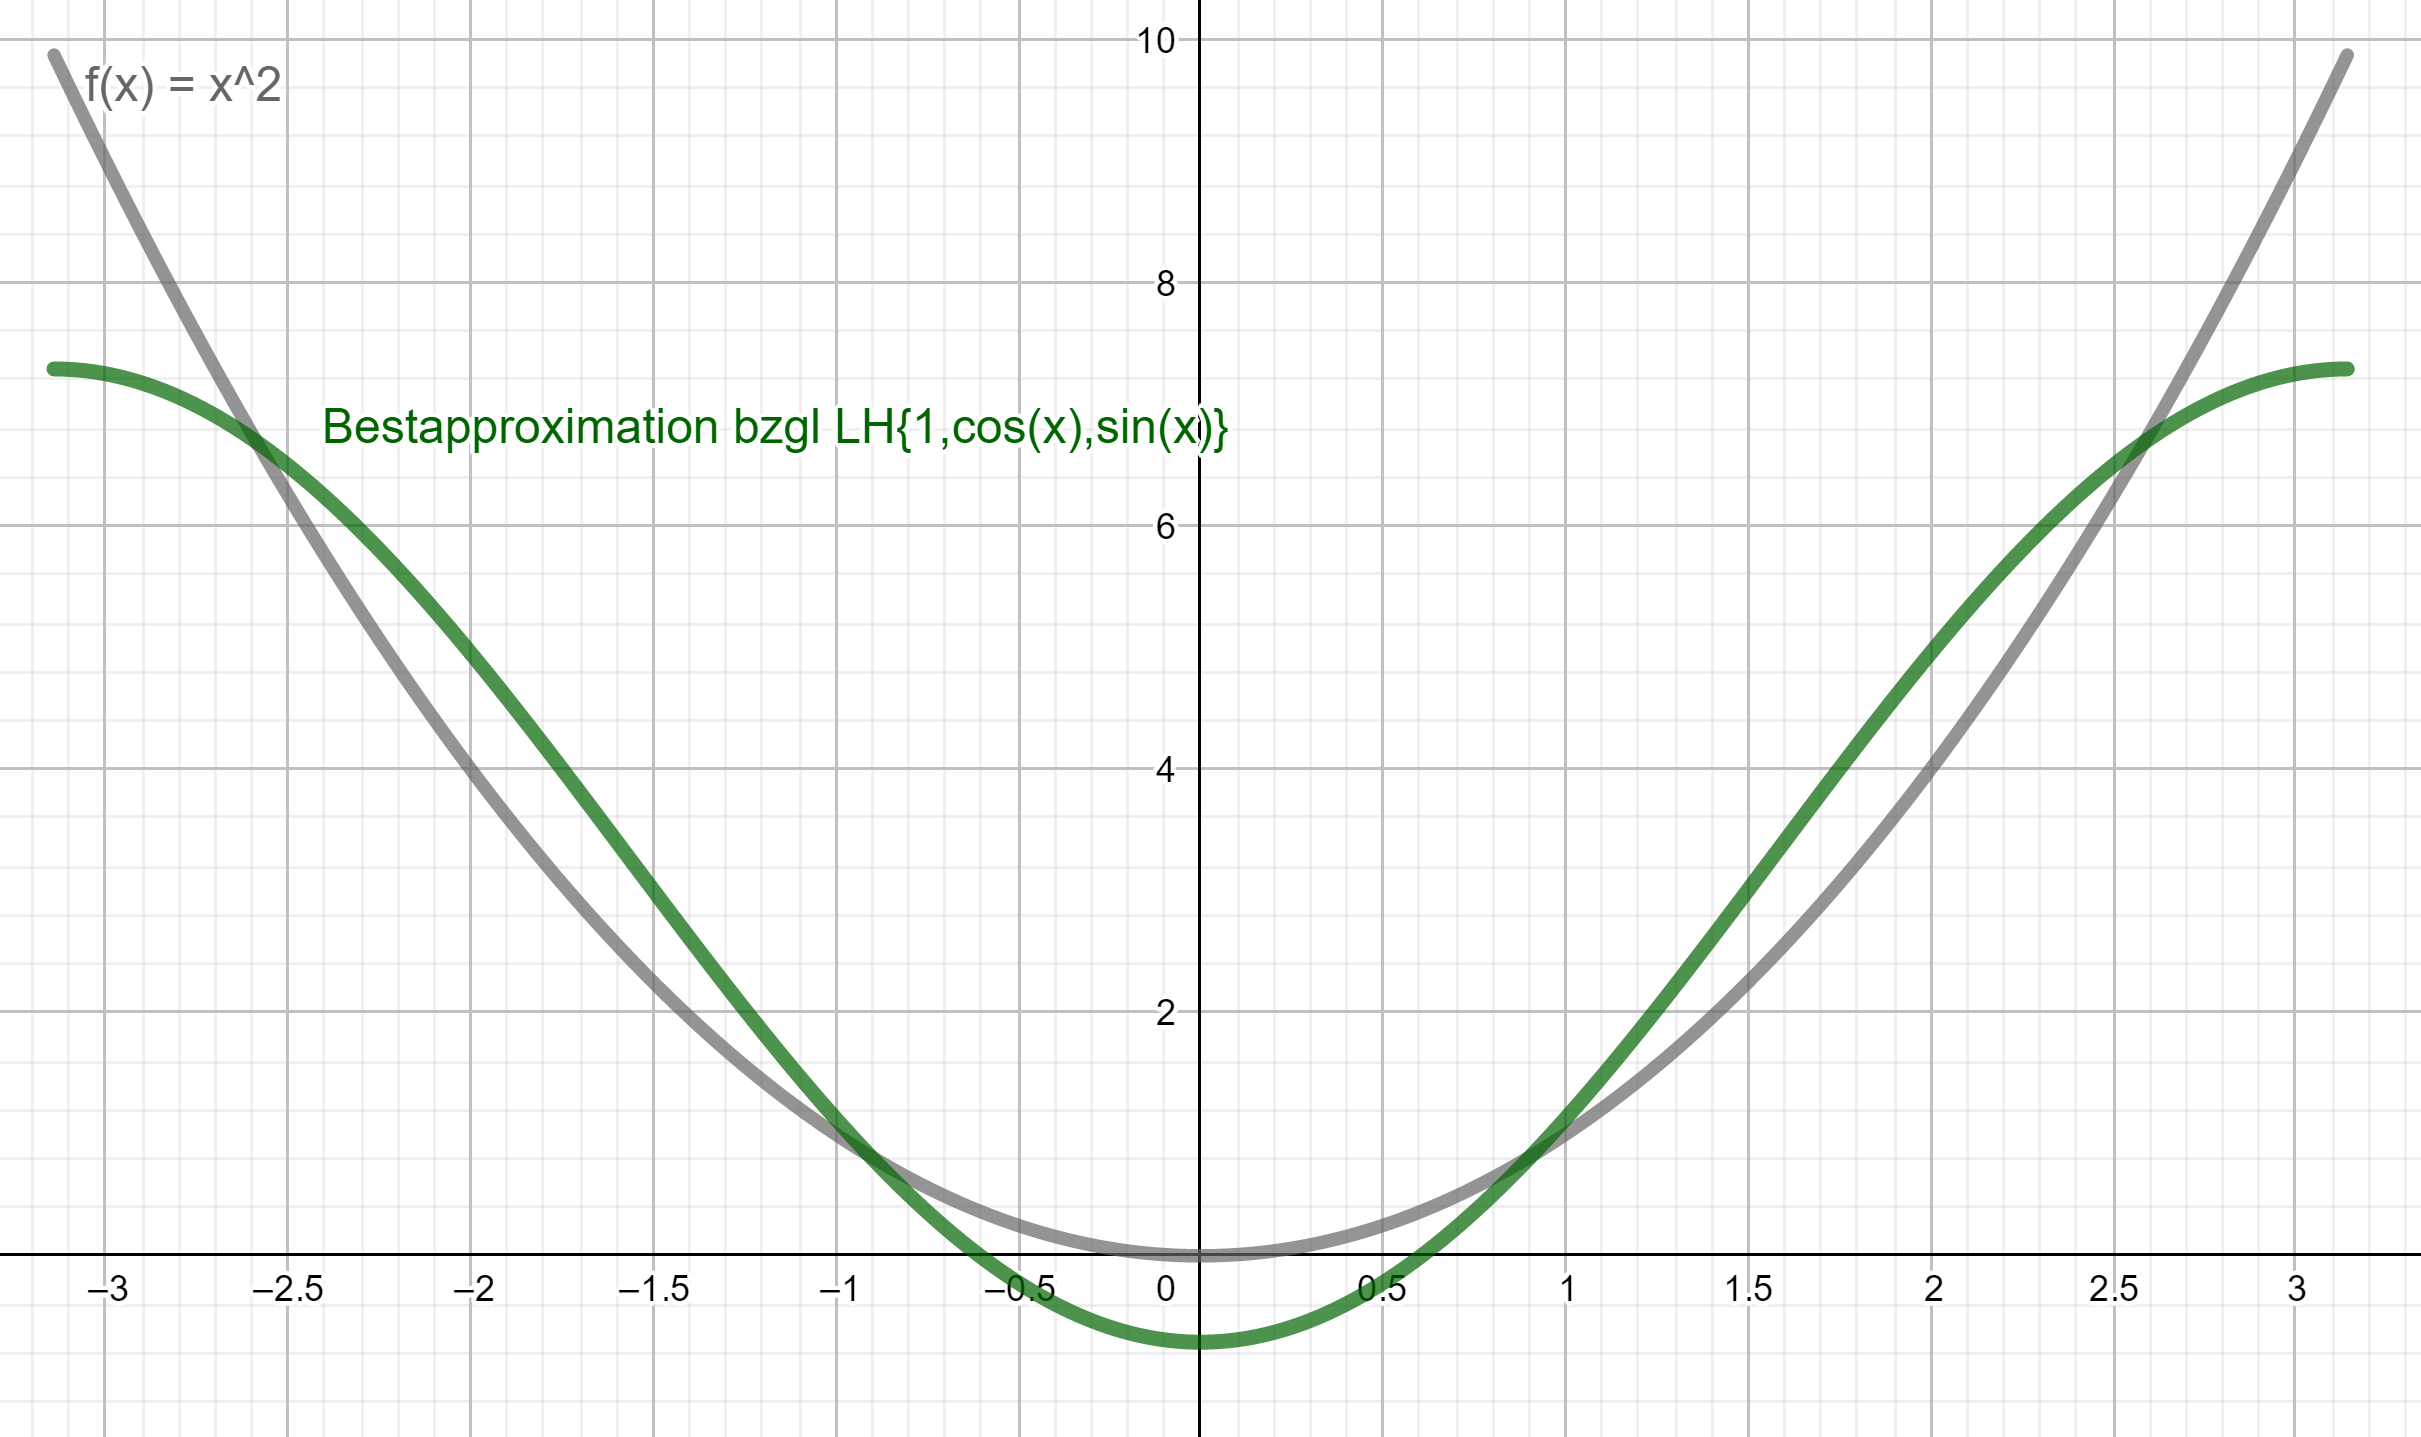
\includegraphics[width=0.8\textwidth]{../Mathematik_2/Bilder/bestapproximation_quadratfunktion_durch_cosinus.png}
\end{center}
	\item[(c)]  Man verwendet die Formeln
		\begin{eqnarray*}
			\cos(\alpha)\cdot \cos(\beta) &=& \frac12 \left( \cos( \alpha - \beta) + \cos(\alpha + \beta)\right) \\
			\sin(\alpha)\cdot \sin(\beta) &=& \frac12 \left( \cos( \alpha - \beta) - \cos(\alpha + \beta)\right) \\
			\sin(\alpha)\cdot \cos(\beta) &=& \frac12 \left( \sin( \alpha - \beta) + \sin(\alpha + \beta)\right)
		\end{eqnarray*}
	\end{itemize}
\end{exercisebox}


\begin{exercisebox}[Bestapproximation]
	Wir betrachten \(\mathcal C([-2,2],\mathbb R)$, den Vektorraum der auf \([-2,2]\) stetigen Funktionen, ausgestattet mit der Maximumsnorm.  Zeigen Sie, dass sich $p$ nicht beliebig genau durch die Funktionen
		\[ f_1(x)=1, \quad f_2(x) = e^x,\quad f_3(x)=e^{2x} \]
		approximieren l��t.

\vspace{0.3cm}
\textbf{L�sung:} \newline
		Offensichtlich liegt $p$ in einem $2$-dimensionalen Unterraum von $\mathcal C([-2,2],\mathbb R)$ und gegeben sind drei linear unabh�ngige Funktionen. W�re $p$ beliebig gut bez�glich der Maximumsnorm approximierbar, dann m�sste sich $p$ also exakt darstellen lassen bez�glich der gegebenen $f_i, i=1,2,3,4$, das hei�t
		\[
		\forall x\in [-2,2]:\quad  x^3-x \stackrel{!}{=} a_0 + a_1e^x + a_2 e^{2x}
	\]
	Es gen�gt eine Auswahl von drei Stellen $x\in [-2,2]$ und wir k�nnen ein lineares Gleichungssystem aufstellen die Zerlegungskoeffizienten $a_i, \, i=0,1,2$ bestimmen. Besonders einfach sind die Nullstellen von $p$: $x_1= 0, x_2 = 1, x_3=-1$.
 \begin{eqnarray*}
	 \begin{cases} 0 \stackrel{!}{=} a_0 + a_1 + a_2 \\
		 0 \stackrel{!}{=} a_0 + a_1 e + a_2 e^2 \\
		 0 \stackrel{!}{=} a_0 + a_1 e^{-1} + a_2 e^{-2}
	 \end{cases}\quad \Rightarrow
	 \left(\begin{array}{ccc|c} 1 & 1 & 1 & 0 \\ 1 & e & e^2 & 0 \\1 e^{-1} & e^{-2} & 0 \end{array}\right) \Leftrightarrow a_i=0, \; i=0,1,2\,.
 \end{eqnarray*}
 Die Approximation ist also $p*: x\mapsto 0$ und damit:
 \[ \| p(x) - p*(x)\|_\infty = 6\,.\]
\end{exercisebox}

